\documentclass{article}
\usepackage{amsfonts}
\usepackage{amssymb}
\usepackage{amsmath}
\usepackage{multicol}
\usepackage[UTF8]{ctex}
\usepackage{tikz}
\usepackage{graphicx}


\usepackage{ifthen}
\newboolean{firstanswerofthesection}  

\usepackage{xcolor}
\colorlet{lightcyan}{cyan!40!white}

\usepackage{chngcntr}
\usepackage{stackengine}

\usepackage{tasks}
\newlength{\longestlabel}
\settowidth{\longestlabel}{\bfseries viii.}
\settasks{counter-format={tsk[r].}, label-format={\bfseries}, label-width=\longestlabel,
    item-indent=0pt, label-offset=2pt, column-sep={10pt}}

\usepackage[lastexercise,answerdelayed]{exercise}
\counterwithin{Exercise}{section}
\counterwithin{Answer}{section}
\renewcounter{Exercise}[section]
\newcommand{\QuestionNB}{\bfseries\arabic{Question}.\ }
\renewcommand{\ExerciseName}{EXERCISES}
\renewcommand{\ExerciseHeader}{\noindent\def\stackalignment{l}% code from https://tex.stackexchange.com/a/195118/101651
    \stackunder[0pt]{\colorbox{cyan}{\textcolor{white}{\textbf{\LARGE\ExerciseHeaderNB\;\large\ExerciseName}}}}{\textcolor{lightcyan}{\rule{\linewidth}{2pt}}}\medskip}
\renewcommand{\AnswerName}{Exercises}
\renewcommand{\AnswerHeader}{\ifthenelse{\boolean{firstanswerofthesection}}%
    {\bigskip\noindent\textcolor{cyan}{\textbf{section \thesection}}\newline\newline%
        \noindent\bfseries\emph{\textcolor{cyan}{\AnswerName\ \ExerciseHeaderNB, page %
                \pageref{\AnswerRef}}}\smallskip}
    {\noindent\bfseries\emph{\textcolor{cyan}{\AnswerName\ \ExerciseHeaderNB, page \pageref{\AnswerRef}}}\smallskip}}
\setlength{\QuestionIndent}{16pt}

\begin{document}
    \section{集合 \& 函数映射}

    \begin{Exercise}
        \vspace{-\baselineskip}% <-- You don't need this line of code if there's some text here

        \Question 将下面韦恩图中的阴影部分用集合 $A, B, C$ 之间的关系式表示出来\underline{\hspace{2cm}}.
        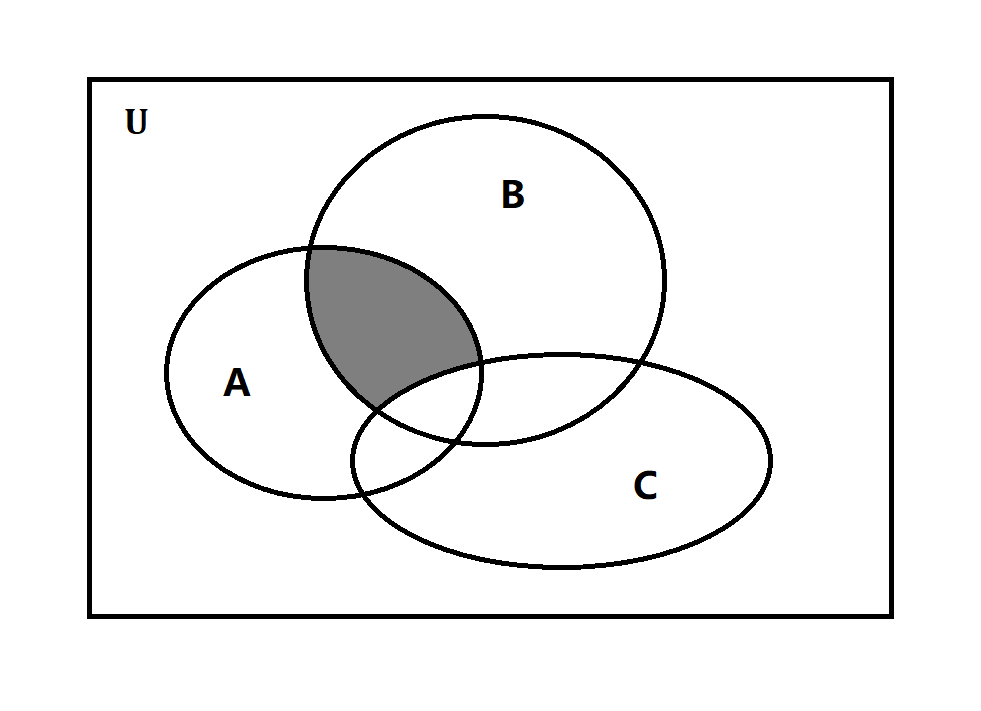
\includegraphics[scale = 0.2]{Sets_internal.png}

        \Question 设集合 $M=\{y|y=2\cos x, x\in[0,5]\}, N=\{x|y=\log_2(x-1)\}$, 则 $M \bigcap N = $(\hspace{1cm}) 
        \begin{tasks}[resume=true](2)
            \task $(-1, 0]$
            \task $(1, 5]$
            \task $[-2, 0]$
            \task $(1, 2]$
        \end{tasks}

        \Question 下图中建立了集合 $P$ 中元素与集合 $M$ 中元素的对应 $f$. 其中为从 $P$ 到 $M$ 的 映射 的
        对应是\underline{\hspace{1.5cm}}, 为从 $P$ 到 $M$ 的 函数 的是\underline{\hspace{1.5cm}}.

        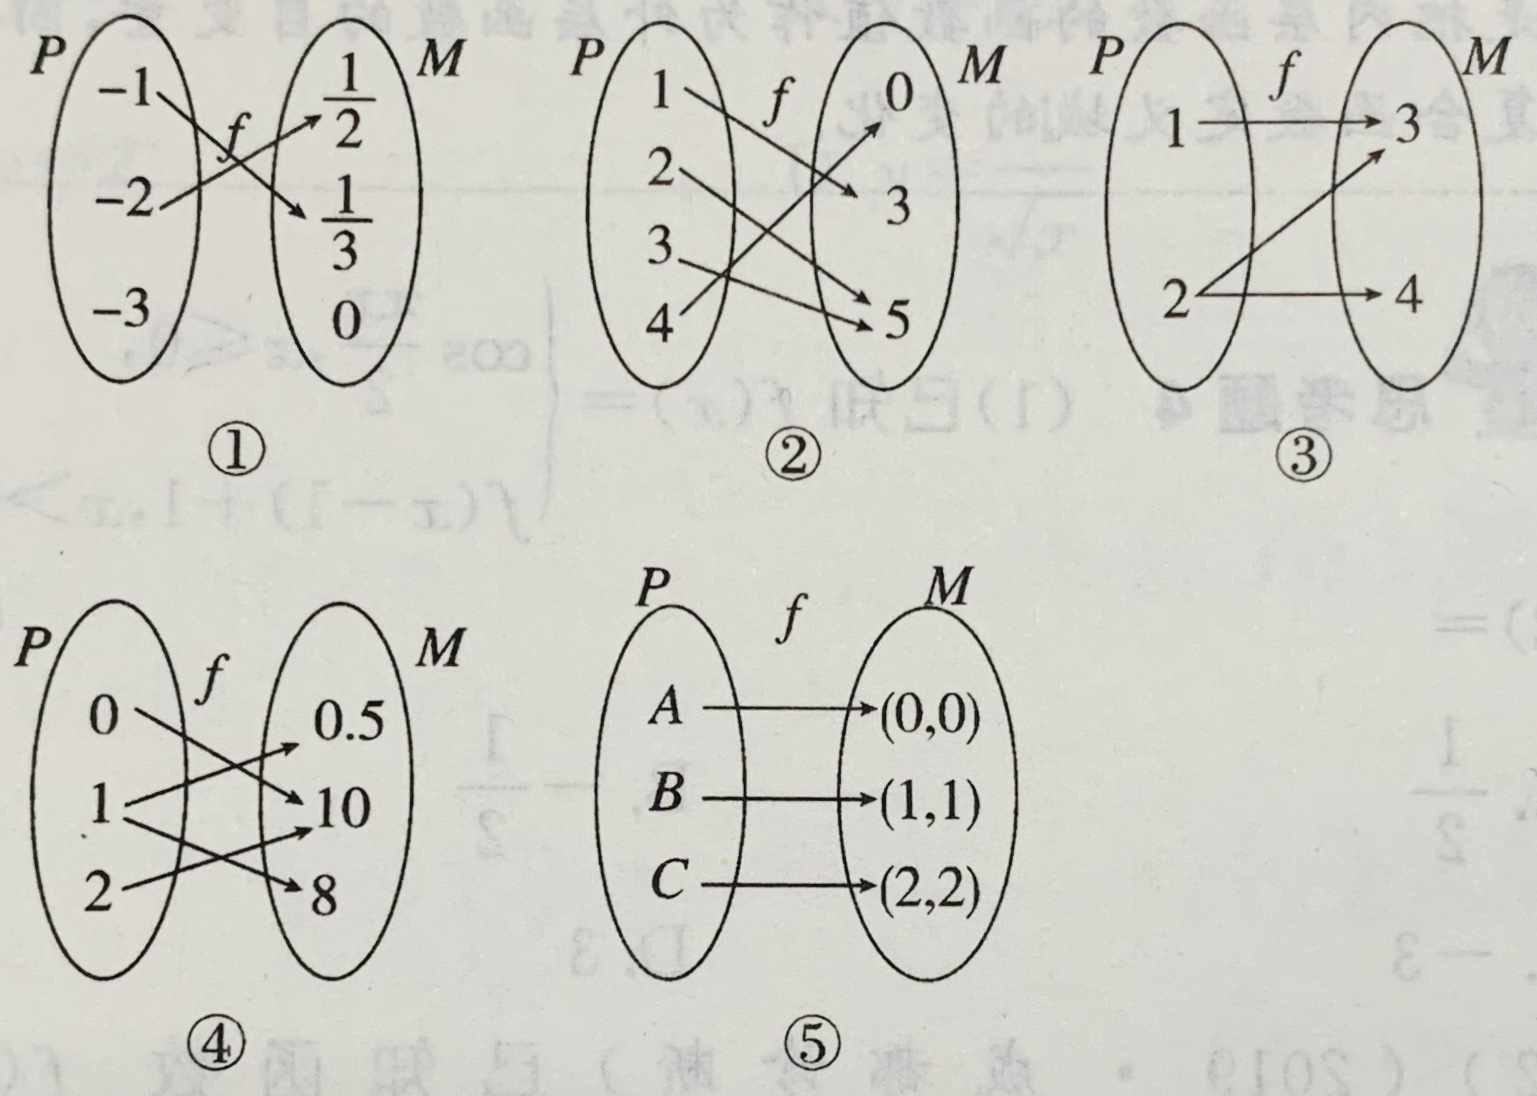
\includegraphics[scale = 0.1]{mapping.png}

        \Question 以下给出函数$f_1, f_2, f_3$, 是否表示同一函数? 

        $ f_1: y = \left\{ \begin{array}{ll}
            1, & x \leqslant 1 \\
            2, & 1 < x <2 \\
            3, & x \geqslant 2 
        \end{array} \right. $
        \hspace{1cm}
        $f_2: $
        \begin{tabular}{|c||c|c|c|}
            \hline
            $x$ & $x \leqslant 1$ &$ 1 < x <2$ & $x \geqslant 2$ \\
            \hline
            $y$ & 1 & 2 & 3 \\
            \hline
        \end{tabular}

        \Question 已知函数 $f(x) = \left\{ \begin{array}{l}
            x-4, x \geqslant 2 \\
            x^2 - 4x + 3, x < 2
        \end{array}\right.$, 求不等式 $f(x) < 0$ 的解集.

    \end{Exercise}
    

\end{document}